\part{Recap on SCMs (+ notation update)}
\frame{\partpage}

\begin{frame}{Structural Causal Models}
  \begin{definition}
  A Structural Causal Model $\C{M}$ is a tuple $\langle \Sin, \Send, \Srnd, \Dom, P, f \rangle$ 
  where
  \begin{itemize}
    \item the \emph{exogenous input variables}, the \emph{endogenous variables} and the \emph{exogenous random variables} are indexed by disjoint (finite) index sets $\Sin, \Send, \Srnd$, respectively;
    \item the \emph{domain} $\Dom = \prod_{i\in \Sin \cup \Send \cup \Srnd} \C{X}_i$ is a product of standard measurable spaces $\C{X}_i$;
    \item the \emph{exogenous distribution} $P$ is a probability distribution on $\CXW$ that factorizes as a product $P = \bigotimes_{k\in\Srnd} P_k$ of probability distributions $P_k \in \C{P}(\C{X}_k)$, one for each exogenous space $\C{X}_k$;
    \item the \emph{causal mechanism} is specified by the measurable function $f : \Dom \to \CXV$.
  \end{itemize}
If $f$ and $P$ depend in a measurable way on \emph{exogenous parameters} $\theta\in\Theta$, 
we write $\C{M}_{\theta} = \langle \Sin, \Send, \Srnd, \Dom, P_{\theta}, f_{\theta} \rangle$.
\end{definition}
In the following slides, fix an SCM $\C{M} = \langle \Sin, \Send, \Srnd, \Dom, P, f \rangle$.
\end{frame}

\begin{frame}{Hard interventions}
  \begin{definition}
  Let $T \subseteq J \cup V \cup W$ be the \emph{intervention target}. We define three variants of \emph{hard interventions}:
    \begin{enumerate}
      \item For a \emph{specified target value} $\xi_T \in \Dom_T$, define
    $$\C{M}_{\doit(X_T=\xi_t)} = \langle J\setminus T, V \cup T, W \setminus T, \Dom, P_{W\setminus T}, (f_{V\setminus T},\xi_T)\rangle$$
  \item For a \emph{stochastic target value} with distribution $Q_T \in \prod_{t\in T} \C{P}(\Dom_t)$, define
    $$\C{M}_{\doit(X_T\sim Q_T)} = \langle J\setminus T, V \setminus T, W \cup T, \Dom, P_{W\setminus T} \otimes Q_T, f_{V\setminus T}\rangle$$
  \item For an \emph{unspecified target value}, define
    $$\C{M}_{\doit(T)} = \langle J\cup T, V\setminus T, W \setminus T, \Dom, P_{W\setminus T}, f_{V\setminus T} \rangle$$
    \end{enumerate}
  \end{definition}
\end{frame}

\begin{frame}{Outcomes and solutions}
\begin{definition}
  Let $\xJ \in \CXJ$ be an input value.
  A pair of random variables $(\XV^{\xJ},\XW)$ with the same domain, and
  respective codomains $\CXV$ and $\CXW$ is called a
  \emph{solution of $\C{M}$ for input $\xJ$} if the following two conditions hold:
    \begin{enumerate}
      \item %its $\Srnd$-component has the exogenous distribution specified by $\C{M}$: 
        $\XW \sim P$ (the exogenous distribution of $\C{M}$),
      \item it satisfies the \emph{structural equations} entailed by $\C{M}$:
        $$\XV^{\xJ} = f\big(\xJ, \XV^{\xJ}, \XW\big) \text{ a.s.}.$$
    \end{enumerate}
 
  For any subset $O \subseteq V \cup W$ that is considered observed, we then call
  $X_O^{\xJ} := (X_{O \cap V}^{\xJ},X_{O \cap W})$ an \emph{(observed) outcome of $\C{M}$ for input $\xJ$}.
\end{definition}
\begin{definition}
  A random field 
  $\Omega \times \CXJ \to \CXV \times \CXW : (\omega,\xJ) \mapsto (\XV^{\xJ}(\omega),\XW(\omega))$
  %with index set $\CXJ$ and codomain $\CXV \times \CXW$ 
  is called a
  \emph{solution of $\C{M}$} if it is measurable and if for all $\xJ\in\CXJ$, $(\XV^{\xJ},\XW)$ is a solution of $\C{M}$ for input $\xJ$.
\end{definition}
\end{frame}

\begin{frame}{Solution function of an SCM}
\begin{definition}
 We call a measurable function
  $g : \CXJ \times \CXW \to \CXV$ a \emph{solution function of $\C{M}$} if it satisfies the structural equations
  for all $\xW\in\CXW$, for all $\xJ\in\CXJ$:
  $$g(\xJ,\xW) = f\big(\xJ, g(\xJ,\xW), \xW\big).$$
\end{definition}
\begin{block}{Remark}
  If $g$ is a solution function for $\C{M}$ then for all random variables $\XW \sim P$,
  the random field $(g(\xJ, \XW), \XW)_{\xJ\in\CXJ}$ is a solution of $\C{M}$,
  and $X_O^{\xJ} := (g_O(\xJ, \XW), X_{O \cap W})$ is an outcome for $\C{M}$ for input $\xJ$.
\end{block}
Not every solution of an SCM can be obtained in this way (e.g., mixtures).
\end{frame}

\begin{frame}{Markov kernel of an SCM solution}
\begin{definition}
  Let $(\XV^{\xJ},\XW)_{\xJ\in\CXJ}$ be a solution of $\C{M}$. 
  %If for each $D \in \Bcal_{\CXV \times \CXW}$ the mapping:
  %      \[ \CXJ \to [0,1],\quad \xJ \mapsto P((\XV^{\xJ},\XW)\in D) \]
  %is measurable, then
  Then
  $$K : \Bcal_{\CXV \times \CXW} \times \CXJ \to [0,1], \quad (D,\xJ) \mapsto P((\XV^{\xJ},\XW)\in D)$$
  is a Markov kernel $\CXJ \dshto \CXV \times \CXW$. We call it a \emph{Markov kernel for $\C{M}$}.

%  If a subset $O \subseteq V \cup W$ is considered observed, we call the marginal kernel
%  $P(X_O \given X_J)$ an \emph{observational Markov kernel of $\C{M}$}.
%
%  For a hard intervention with target $T \subseteq \Sin \cup \Send \cup \Srnd$, we will call a
%  Markov kernel of the intervened SCM $\C{M}_{\doit(T)}$ an \emph{interventional Markov kernel of $\C{M}$}.
\end{definition}
Since in general an SCM may have different solutions, it can also have different Markov kernels.
\end{frame}

\part{Unique solvability and Simple SCMs}
\frame{\partpage}

\begin{frame}{Unique solvability}
\begin{definition}
  $\C{M}$ is called \emph{uniquely solvable} if it has a unique solution function. 
\end{definition}
\begin{example}
  An SCM with endogenous real variables $X,Y$, and exogenous real random variable $E$, and structural equations
  $$X = Y, \qquad Y = X$$
  is not uniquely solvable (since any measurable function $\RN \to \RN^2$ mapping $e$ to an arbitrary value $(x,x)$ is
  a solution function).

  If it had structural equations
  $$X = E, \qquad Y = X$$
  instead, it would be 
  uniquely solvable (since the only measurable solution function is $\RN \to \RN^2 : e \mapsto (e,e)$).
\end{example}
\end{frame}

\begin{frame}{Unique solvability properties}
\begin{theorem}
  \begin{enumerate}
    \item $\C{M}$ is uniquely solvable if and only if 
      for all $\xW\in\CXW$, for all $\xJ \in \CXJ$, the equation
      $$\xV = f(\xV,\xJ,\xW)$$
      has a unique solution for $\xV\in\CXV$.
%    \item If $\C{M}$ is uniquely solvable, then for all $\xJ\in\CXJ$, $\C{M}_{\doit(\XJ=\xJ)}$ is uniquely solvable.
    \item If $\C{M}$ is uniquely solvable, it has a unique Markov kernel
      $$P_{\C{M}}(X_V,X_W \mid \doit(X_J)) := (g,\id_{\CXW})_* \bigotimes_{k\in\Srnd} P_k$$
  \end{enumerate}
\end{theorem}
\begin{definition}
  If a subset of variables $O \subseteq V \cup W$ is considered observed, its marginal
  $P_{\C{M}}(X_O \mid \doit(X_J))$ is called the \emph{observational Markov kernel of $\C{M}$}.
\end{definition}
\end{frame}

\begin{frame}{Proof ideas}
  \begin{enumerate}
    \item Apart from checking the definitions, we have to prove that the solution function is measurable.
This follows (with some more advanced measure theory) from the measurability of the causal mechanism $f$.

    \item Let $g : \CXJ \times \CXW \to \CXV$ be the unique solution function of $\C{M}$.
      The Markov kernel is obtained as the push-forward
      $$P_{\C{M}}(\XV,\XW \mid \XJ) = (g,\id_{\CXW})_* P(\XW \mid \XJ)$$
      of the exogenous distribution of $\C{M}$, interpreted as a constant Markov kernel $\CXJ \dshto \CXW$:
  $$P(\XW \mid \XJ) := \bigotimes_{k\in\Srnd} P(X_k).$$
  Equivalently, for all $\xJ \in \XJ$,
      $$P_{\C{M}}(\XV,\XW \mid \XJ=\xJ) = P((g(\xJ,\XW),\XW))$$
      for a random variable $\XW \sim P$. The uniqueness of $P_{\C{M}}$ follows eventually from the uniqueness of $g$.
  \end{enumerate}
\end{frame}

\begin{frame}{Simple SCMs}
For simplicity, we consider mostly ``simple SCMs'':
\begin{definition}
  An SCM $\C{M}$ is called \emph{simple} if the intervened SCM
  $\C{M}_{\doit(T)}$ is uniquely solvable for all $T \subseteq \Sin \cup \Send \cup \Srnd$. 
\end{definition}
Note that this includes unique solvability of $\C{M}$ itself for $T = \emptyset$.
\begin{corollary}
  If $\C{M}$ is simple, and $O \subseteq V \cup W$ is considered observed, then for all $T \subseteq O$, the
  observational Markov kernel $P_{\C{M}}(X_O \mid \doit(X_J))$
  and all its \emph{interventional Markov kernels}
  $$P_{\C{M}}(X_{O\setminus T} \mid \doit(X_J),\doit(X_T)) := P_{\C{M}_{\doit(T)}}(X_{O\setminus T} \mid \doit(X_{J \cup T}))$$
  exist and are unique.
\end{corollary}
\end{frame}

\begin{frame}{Example of simple SCM}
\begin{example}
Consider an SCM with structural equations
$$X_1 = W_1 \qquad X_2 = W_2 \qquad X_3 = X_1 X_4 + W_3 \qquad X_4 = X_2 X_3 + W_4 $$
where the $X$'s are considered endogenous real variables and the $W$'s exogenous variables with domains $(-1,1)$.
We can solve the system of structural equations with respect to $X$ in terms of $W$:
$$X_1 = W_1 \qquad X_2 = W_2 \qquad X_3 = \frac{W_3 + W_1 W_4}{1 - W_1 W_2} \qquad X_4 = \frac{W_2 W_3 + W_4}{1 - W_2 W_1}$$
Similarly, we can take any subset of the structural equations and solve it with respect to the variables appearing on the l.h.s.\ in terms of the variables appearing on the r.h.s.\ of the equations in the subset, and obtain a unique solution. Thus this SCM is simple.
%For example, only solving the structural equations for $X_3$ and $X_4$, we obtain:
%$$X_3 = \frac{W_3 + W_1 W_4}{1 - W_1 X_2} \qquad X_4 = \frac{W_2 W_3 + W_4}{1 - W_2 X_1}$$
%where the variables $X_1$ and $X_2$ are now considered as exogenous input variables (instead of endogenous variables).
%Hence, any subset of the structural equations has a unique solution for the variables appearing on the l.h.s.\ in terms
%of the remaining ones on the r.h.s., which means that this SCM is simple.
\end{example}
We will see later that all acyclic SCMs are simple.
\end{frame}

\begin{frame}{Relations between causal models}
  \centerline{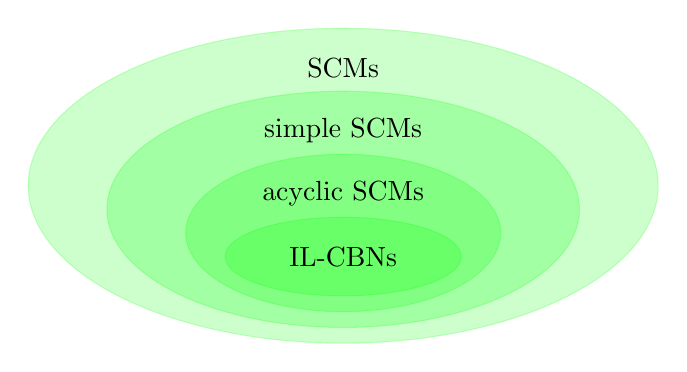
\begin{tikzpicture}
      \begin{scope}
        \draw[draw=green,fill=green,opacity=0.2] (0,0) ellipse (1.5cm and 0.5cm);
        \draw[draw=green,fill=green,opacity=0.2] (0,0.3) ellipse (2cm and 1cm);
        \draw[draw=green,fill=green,opacity=0.2] (0,0.6) ellipse (3cm and 1.5cm);
        \draw[draw=green,fill=green,opacity=0.2] (0,0.9) ellipse (4cm and 2cm);
        \node at (0,0) {IL-CBNs};
        \node at (0,0.8) {acyclic SCMs};
        \node at (0,1.6) {simple SCMs};
        \node at (0,2.4) {SCMs};
      \end{scope}
  \end{tikzpicture}}

  \bigskip
  Simple SCMs are more expressive than IL-CBNs, because they:
  \begin{enumerate}
    \item Encode counterfactuals
    \item Can model causal cycles (e.g., feedback loops)
  \end{enumerate}
\end{frame}

\part{Counterfactuals}
\frame{\partpage}

\begin{frame}{Informal definition}
  \begin{definition}[Informal]
Counterfactuals are hypothetical statements regarding the effects of some change that is contrary-to-fact.
  \end{definition}

  A counterfactual statement invites one to imagine an alternative (counterfactual) world, in which 
  everything is the same as in the actual world, except that one aspect of it is changed.
  We use our causal model of the world to predict the consequences of this imaginary change.

  \begin{example}
  Suppose you are healthy but drank too much beer last night and now suffer from a hangover. 
  A counterfactual statement is then: ``If I had not drunk so much beer yesterday, I would feel much better now.''
  \end{example}

  Counterfactual thinking is very common in humans, and toddlers already bombard
  their parents with counterfactual questions, presumably as a means for them
  to build internal causal models of the world.
\end{frame}

\begin{frame}{Twin SCM}
\begin{definition}
  We define the \emph{twinned SCM} $\C{M}^\twin = \langle \Sin \dot\cup \Sin', \Send \dot\cup \Send', \Srnd, \tilde{\Dom}, P, \tilde{f} \rangle$
  with 
  \begin{enumerate}
    \item $\Sin' = \{j' : j \in \Sin\}$ a copy of $\Sin$,
    \item $\Send' = \{v' : v \in \Send\}$ a copy of $\Send$, 
    \item the twinned domain given by
  $$\tilde{\Dom} = \CXJ \times \CXJ \times \CXV \times \CXV \times \CXW$$
  (i.e., with $\Dom_{\Sin'} = \Dom_{\Sin}$ and $\Dom_{\Send'} = \Dom_{\Send}$),
    \item the twinned causal mechanism components given by
  $$\tilde{f}_v\big((x_J,x_{J'}),(x_V,x_{V'}),\xW\big) = 
  \begin{cases}
    f_v(\xJ,\xV,\xW) & v \in \Send,  \\
    f_v(x_{J'},x_{V'},\xW) & v \in \Send'.
  \end{cases}$$
  \end{enumerate}
\end{definition}
  This creates copies of some variables so that their values can differ in the counterfactual world with respect to the actual world.
\end{frame}

\begin{frame}{Counterfactuals: Example}
  \begin{example}
  Variables:\\
    \quad $T$ : number of hours studied (exogenous input variable)\\
    \quad $E$ : study efficiency (exogenous input variable)\\
    \quad $D$ : exam difficulty (exogenous random variable)\\
    \quad $G$ : grade (endogenous variable)\\
  Structural equation:\\
  \smallskip
  \centerline{$G = f(T,D,E).$}
  \smallskip
  Counterfactual query: {\it ``I studied 20 hours for the exam and
got a 4.5; if I had studied 30 hours instead, what would have been my grade?''}\\

    \medskip
    Twin SCM has copies $T'$, $E'$ and $G'$, and structural equations:\\
    \smallskip
    \centerline{$G = f(T,D,E) \qquad G' = f(T',D,E').$}
    \smallskip
    The answer to the counterfactual query is:\\
    \smallskip
    \centerline{$P(G' \given \doit(E=e), \doit(E'=e), \doit(T'=30), \doit(T=20), G=4.5)$}
    \smallskip
  \end{example}
\end{frame}

\begin{frame}{Discussion}
The English language has a grammatical construct for counterfactuals:\\
\quad ``If I had studied better, I would have passed the exam,''\\
instead of\\
\quad ``If I study well, I will pass the exam.''\\
For the former statement, we first twin the SCM and then intervene on it, for the latter, we only intervene on the SCM (no need for twinning!). 

\bigskip
So not only from the grammatical, but also from the modeling point of view, these are quite different questions!

\bigskip
\setbeamercolor{block title}{use=structure,fg=white,bg=purple!75!black}
\setbeamercolor{block body}{use=structure,fg=black,bg=white!20!white}
  \begin{block}{Warnings}
    \begin{itemize}
      \item
  Unfortunately, in large part of the causality literature, the term ``counterfactuals'' is also used 
  as a synonym for potential outcomes, which are not necessarily contrary-to-fact. This may
  cause confusion.
%  (for example, ``If you drink too much beer you will get a hangover'').
\item Generally, in situations where the full causal mechanism is unknown, or exogenous
randomness is latent, counterfactuals may be very model-dependent.
    \end{itemize}
  \end{block}
\end{frame}

\part{Important Equivalence Relations}
\frame{\partpage}

\begin{frame}{Pearl's Ladder of Causation}
  \centering
  \begin{tikzpicture}
    \node (0,0) {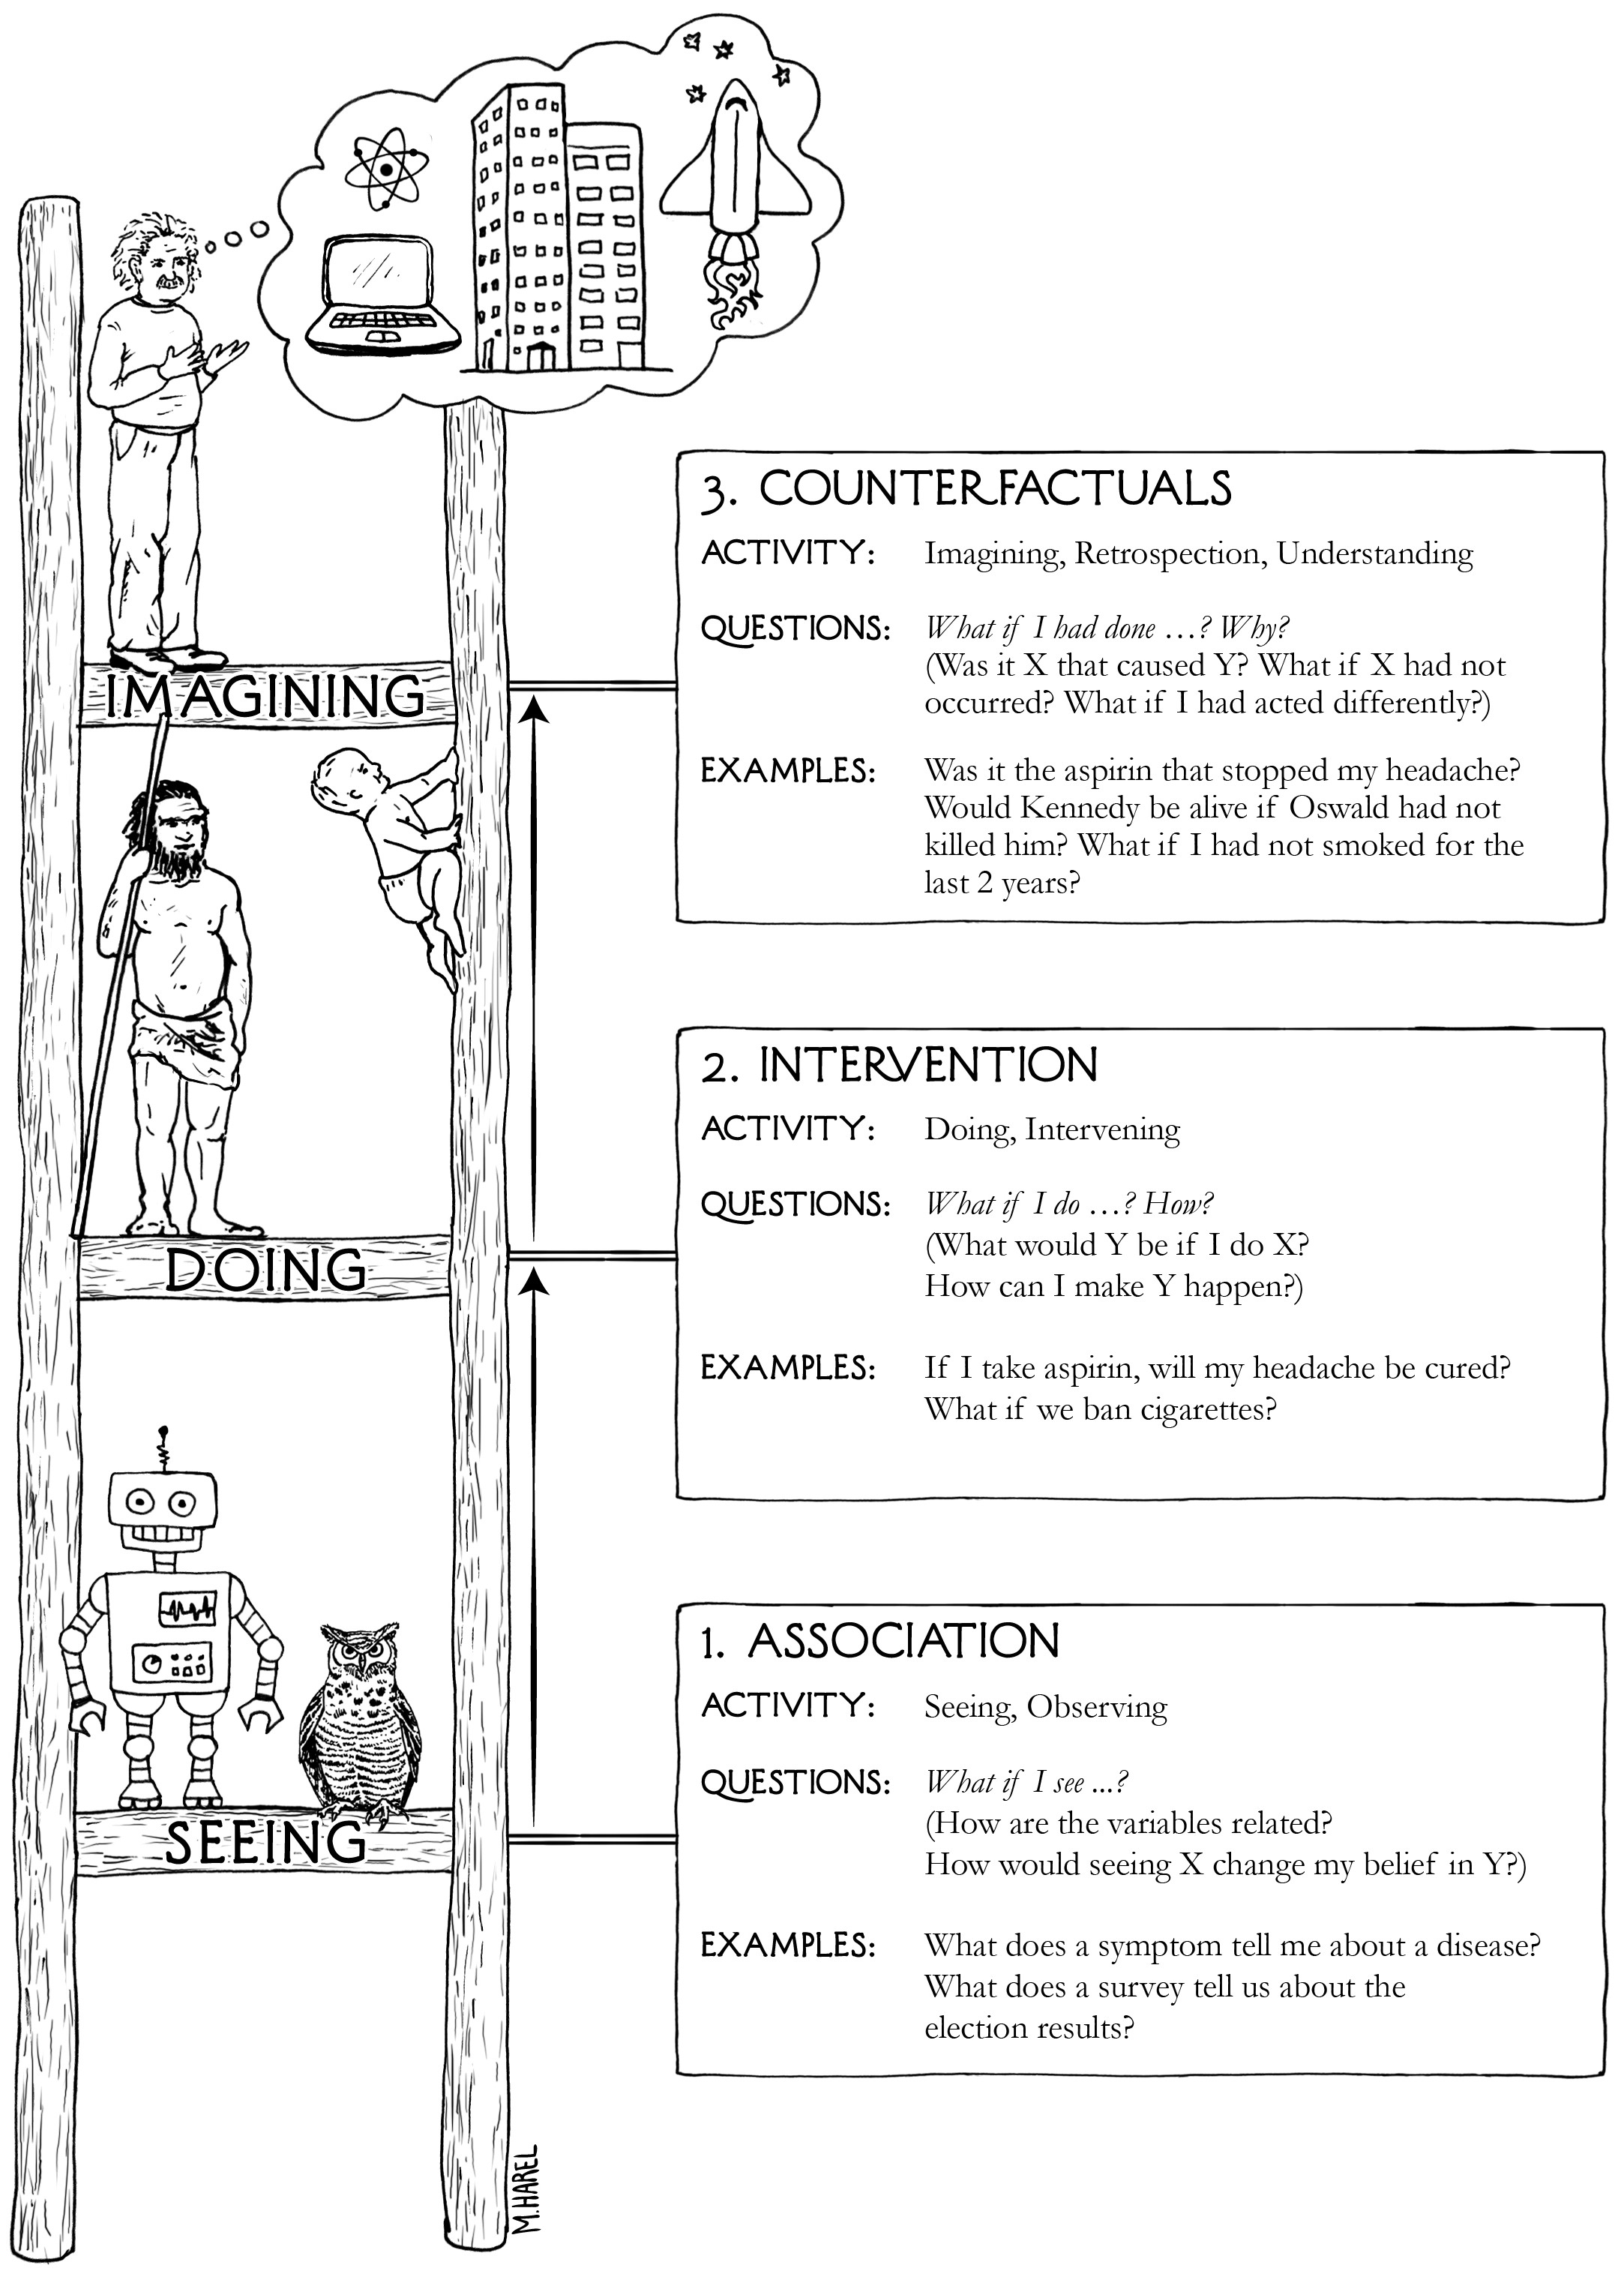
\includegraphics[width=0.45\textwidth]{ladder.jpg}};
    \draw[line width=1mm,fill=green,draw=green,->] (-4,2) -- node[below,sloped] {data-driven} (-4,-2);
    \draw[line width=1mm,fill=red,draw=red,->] (4,-2) -- node[below,sloped] {model-based} (4,2);
  \end{tikzpicture}
  \centerline{\tiny Image from Pearl \& Mackenzie, {\it The Book of Why}}
\end{frame}

\begin{frame}{Equivalence relations}
Equivalence relations capture the notion that mathematical objects can be ``equivalent'' from some point of view.
\begin{definition}
  Let $Z$ be a set and $R \subseteq Z^2$ be a relation on $Z$ (i.e., a subset of ordered pairs of $Z$). $R$ is called an \emph{equivalence relation} if 
  \begin{enumerate}
    \item $R$ is reflexive: $(a,a) \in R$ for all $a \in Z$;
    \item $R$ is symmetric: $(a,b) \in R \iff (b,a) \in R$ for all $a,b \in Z$;
    \item $R$ is transitive: if $(a,b) \in R$ and $(b,c) \in R$ then $(a,c) \in R$ for all $a,b,c\in Z$.
  \end{enumerate}
\end{definition}
\end{frame}

\begin{frame}{Equivalence of SCMs}
\begin{definition}
  Let $\C{M} = \langle \Sin, \Send, \Srnd, \Dom, P, f \rangle$ and
  $\tilde{\C{M}} = \langle \Sin, \Send, \Srnd, \Dom, P, \tilde{f} \rangle$ be two SCMs.
  We say that
  $\C{M}$ is \emph{equivalent} to $\tilde{\C{M}}$ and write $\C{M} \equiv \tilde{\C{M}}$ if for each $v \in \Send$,
  $$\forall x \in \Dom: \quad x_v = f_v(\xJ,\xV,\xW) \iff x_v = \tilde{f}_v(\xJ,\xV,\xW).$$
%  In words, $\C{M}$ and $\tilde{\C{M}}$ are considered equivalent if they at most differ in terms of their
%  causal mechanisms, yet each of their structural equations has the same solutions.
\end{definition}
\begin{block}{Proposition}
\begin{enumerate}
  \item Equivalence of SCMs is preserved by hard interventions.
  \item Equivalence of SCMs is preserved by twinning.
  \item Unique solvability and simplicity are invariants of SCM equivalence.
  \item Equivalent SCMs have the same solution functions, solutions, (potential) outcomes, and (observational and interventional) Markov kernels.
\end{enumerate}
\end{block}
\end{frame}

\begin{frame}{Example of equivalent SCMs}
\begin{example}
  The SCM with the single structural equation
  $$X = -X^3 + X + W$$
  where $X$ is endogenous, and $W$ is exogenous, is equivalent to the SCM obtained by replacing the structural equation with
  $$X = \sqrt[3]{W}.$$
  Note that $X$ no longer appears on the r.h.s..
\end{example}
\end{frame}

\begin{frame}{Other equivalences: definition}
\begin{definition}
  Let $\C{M} = \langle \Sin, \Send, \Srnd, \Dom, P, f \rangle$ and
  $\tilde{\C{M}} = \langle \tilde{\Sin}, \tilde{\Send}, \tilde{\Srnd}, \tilde{\Dom}, \tilde{P}, \tilde{f} \rangle$ be two simple SCMs
  and $O \subseteq (\Send \cap \tilde{\Send}) \cup (\Srnd \cap \tilde{\Srnd})$ a subset.
  We say that:
  \begin{enumerate}
    \item $\C{M}$ and $\tilde{\C{M}}$ are \emph{observationally equivalent w.r.t.\ $O$} if $\Dom_O = \tilde{\Dom}_O$, $J = \tilde{J}$, $\Dom_J = \tilde{\Dom}_J$ and $P_{\C{M}}(X_O \mid \doit(\XJ)) = P_{\tilde{\C{M}}}(X_O \mid \doit(\XJ))$;
    \item $\C{M}$ and $\tilde{\C{M}}$ are \emph{interventionally equivalent w.r.t.\ $O$} if for every subset $T \subseteq O$ the intervened SCMs $\C{M}_{\doit(T)}$ and $\tilde{\C{M}}_{\doit(T)}$ are observationally equivalent w.r.t.\ $O \setminus T$;
    \item $\C{M}$ and $\tilde{\C{M}}$ are said to be \emph{counterfactually equivalent w.r.t.\ $O$} if the twin SCMs $\C{M}^\twin$ and $\tilde{\C{M}}^\twin$ are interventionally equivalent w.r.t.\ $O \cup O'$, where
  $O'$ is the copy of $O$ in $\Send' \cap \tilde{\Send}'$.
  \end{enumerate}
  In case the variables in $(V \cup W) \setminus O$ are considered latent, we sometimes omit the ``w.r.t.\ $O$'' in this terminology (i.e., we call $\C{M}$ and $\tilde{\C{M}}$ observationally equivalent, interventionally equivalent and counterfactually equivalent, respectively).
\end{definition}
\end{frame}

\begin{frame}{Other equivalences: relationships}
\begin{block}{Proposition}
  For simple SCMs $\C{M}, \tilde{\C{M}}$ and a subset $O \subseteq (\Send \cap \tilde{\Send}) \cup (\Srnd \cap \tilde{\Srnd})$:
  \begin{enumerate}
    \item If $\C{M} \equiv \tilde{\C{M}}$ then $\C{M}$ and $\tilde{\C{M}}$ are counterfactually equivalent w.r.t.\ $O$.
    \item If $\C{M}$ and $\tilde{\C{M}}$ are counterfactually equivalent w.r.t.\ $O$ then 
      $\C{M}$ and $\tilde{\C{M}}$ are interventionally equivalent w.r.t.\ $O$.
    \item If $\C{M}$ and $\tilde{\C{M}}$ are interventually equivalent w.r.t.\ $O$ then 
      $\C{M}$ and $\tilde{\C{M}}$ are observationally equivalent w.r.t.\ $O$.
  \end{enumerate}
\end{block}
The reverse implications do not hold in general. This expresses that causal modeling is more refined than
probabilistic modeling, and counterfactual modeling is more refined than interventional modeling.
\end{frame}

\begin{frame}{Counterexample 1}
\begin{example}
  The following SCMs are both simple:
  \begin{align*}
    \C{M} &: \qquad N \sim \C{N}(\mu,\sigma^2) \qquad C = \alpha + \beta N \\
    \tilde{\C{M}}&: \qquad C \sim \C{N}(\tilde{\mu},\tilde{\sigma}^2) \qquad N = \tilde{\alpha} + \tilde{\beta} C
  \end{align*}
Their observational distributions are respectively 
  $$P(N,C) = \C{N}\left(\begin{pmatrix} \mu \\ \alpha \mu \end{pmatrix}, \begin{pmatrix} \sigma^2 & \beta\sigma^2 \\ \beta\sigma^2 & \beta^2\sigma^2\end{pmatrix}\right)$$
and
  $$P(N,C) = \C{N}\left(\begin{pmatrix} \tilde{\alpha}\tilde{\mu} \\ \tilde{\mu} \end{pmatrix}, \begin{pmatrix} \tilde{\beta}^2\tilde{\sigma}^2 & \tilde{\beta}\tilde{\sigma}^2 \\ \tilde{\beta}\tilde{\sigma}^2 & \tilde{\sigma}^2\end{pmatrix}\right)$$
For certain parameter choices, they are observationally equivalent.
They are NOT interventionally equivalent except for very special parameter choices.
\end{example}
\end{frame}

\begin{frame}{Counterexample 2 (Dawid, 2002)}
\begin{example}[1/2]
  For parameter $\rho\in[0,1]$, consider the SCM $\C{M}_\rho$ with binary exogenous input variable $X \in \{0,1\}$, endogenous variable $Y$, a single latent exogenous random variable $W = (W_1,W_2) \in \RN^2$ with
exogenous distribution 
  $$\begin{pmatrix} W_1 \\ W_2 \end{pmatrix}\sim\C{N}\left(\begin{pmatrix}0 \\ 0\end{pmatrix},\begin{pmatrix}1&\rho\\ \rho&1\end{pmatrix}\right)$$
and structural equation
  $$Y = W_1 (1 - X) + W_2 X.$$
In a medical setting, this SCM could be used to model whether a patient was treated ($X$) and the corresponding outcome for that patient ($Y$).
\end{example}
\end{frame}

\begin{frame}{Counterexample 2 (Dawid, 2002)}
\begin{example}[2/2]
  Suppose in the actual world, $X = 0$ and $Y^0 = y \in \RN$.
  Consider the counterfactual: {\it ``What would the outcome have been, had we assigned treatment to this patient?''}.

  Construct the twin SCM $\C{M}_{\rho}^{\twin}$.
The counterfactual query then asks for $P((Y')^1=y'\mid Y^0=y)$. One can calculate that
$$
  P\big((Y')^1,Y^0\big) = \C{N}\left(\begin{pmatrix}0\\ 0\end{pmatrix}, \begin{pmatrix} 1 & \rho \\ \rho & 1 \end{pmatrix}\right)
$$
and hence $P((Y')^1 \mid Y^0=y) = \C{N}(\rho y,1-\rho^2)$. Note that the answer to the counterfactual query depends on a quantity $\rho$ that we cannot identify from the Markov kernel $P(Y\given \doit X)$, since this is independent of $\rho$. 
Indeed, SCMs $\C{M}_{\rho}$ and $\C{M}_{\rho'}$ with $\rho\neq\rho'$ are interventionally equivalent, but not counterfactually equivalent.
%If we obtain the SCM from a reduction, we find the one with $\rho = 1$.
\end{example}
\end{frame}
